%
% teil1.tex -- Beispiel-File für das Paper
%
% (c) 2020 Prof Dr Andreas Müller, Hochschule Rapperswil
%
\section{Beispiel ()
\label{lambertw:section:teil1}}
\rhead{Problemstellung}



%\begin{figure}[H]
%	\centering
%	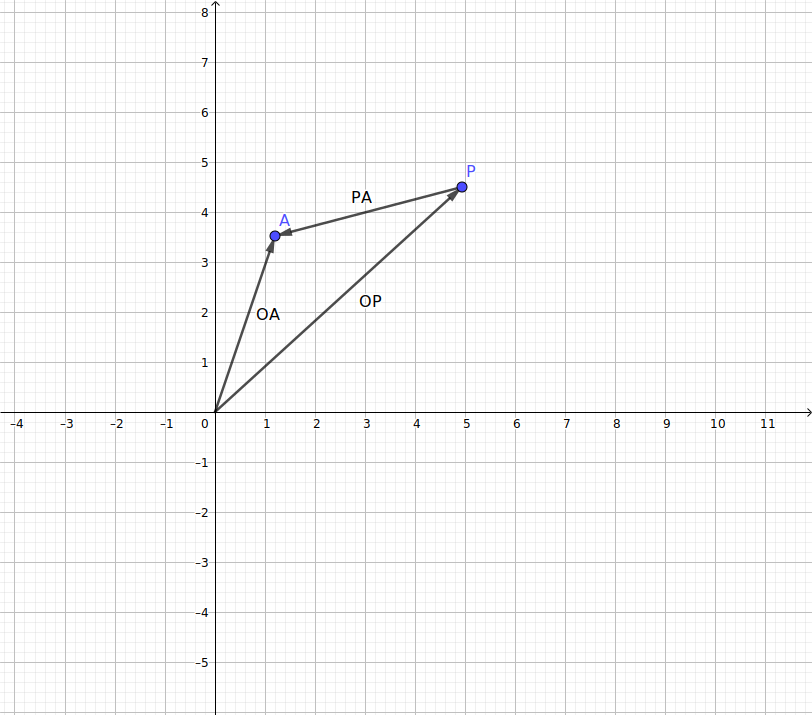
\includegraphics[width=0.5\textwidth]{.\Bilder\something.pdf}
%   \label{pursuer:grafik1}
%\end{figure}



Je nach Verfolgungsstrategie die der Verfolger verwendet, entsteht eine andere DGL.
Für dieses konkrete Beispiel wird einfachheitshalber die simpelste Strategie gewählt.
Bei dieser Strategie bewegt sich der Verfolger immer direkt auf sein Ziel hinzu.
Womit der Geschwindigkeitsvektor des Verfolgers zu jeder Zeit direkt auf das Ziel zeigt.

Um die DGL dieses Problems herzuleiten wird der Sachverhalt in der Grafik \eqref{pursuer:grafik1} aufgezeigt.
Der Punkt $P$ ist der Verfolger und der Punkt $A$ ist sein Ziel.

Um dies mathematisch beschreiben zu können, wird der Richtungsvektor
\begin{equation}
    \frac{A-P}{|A-P|}
    =
    \frac{\dot{P}}{|\dot{P}|}
\end{equation}
benötigt. Durch die Subtraktion der Ortsvektoren $\overrightarrow{OP}$ und $\overrightarrow{OA}$ entsteht ein Vektor der vom Punkt $P$ auf $A$ zeigt.
Da die Länge dieses Vektors beliebig sein kann, wird durch Division mit dem Betrag, die Länge auf eins festgelegt.
Aus dem Verfolgungsproblem ist auch ersichtlich, dass die Punkte $A$ und $P$ nicht am gleichen Ort starten und so eine Division durch Null ausgeschlossen ist.
Wenn die Punkte $A$ und $P$ trotzdem am gleichen Ort starten, ist die Lösung trivial.

Nun wird die Gleichung mit deren rechten Seite skalar multipliziert, um das Gleichungssystem von zwei auf eine Gleichung zu reduzieren.
\begin{equation}
    \label{pursuer:pursuerDGL}
    \frac{A-P}{|A-P|}\cdot \frac{\dot{P}}{|\dot{P}|}
    =
    1
\end{equation}
Diese DGL ist der Kern des Verfolgungsproblems, insofern sich der Verfolger immer direkt auf sein Ziel zubewegt.


\subsection{Beispiel}
Das Verfolgungsproblem wird mithilfe eines konkreten Beispiels veranschaulicht. Dafür wird die einfachste Strategie verwendet, bei der sich der Verfolger direkt auf sein Ziel hinzu bewegt. Für dieses Problem wurde bereits die DGL \eqref{pursuer:pursuerDGL} hergeleitet.

Um dieses Beispiel einfach zu halten, wird für den Verfolger und das Ziel jeweils eine konstante Geschwindigkeit von eins gewählt. Das Ziel wiederum startet im Ursprung und bewegt sich linear auf der positiven Y-Achse.

\begin{align}
    v_P^2
    &=
    \dot{P}\cdot\dot{P}
    =
    1
    \\[5pt]
    v_A
    &=
    1
    \\[5pt]
    A
    &=
    \begin{pmatrix}
    	0 \\
    	v_A\cdot t
    \end{pmatrix}
	=
	\begin{pmatrix}
		0 \\
		t
	\end{pmatrix}
	\\[5pt]
	P
	&=
	\begin{pmatrix}
		x \\
		y
	\end{pmatrix}
\end{align}

Die Anfangsbedingungen dieses Problems sind.

\begin{align}
	y(t)\bigg|_{t=0}
	&=
	y_0
	\\[5pt]
	x(t)\bigg|_{t=0}
	&=
	x_0 \\[5pt]
	\frac{\,dy}{\,dx}(t)\bigg|_{t=0}
	&=
	\frac{y_A(t) -y_P(t)}{x_A(t)-x_P(t)}\bigg|_{t=0}
\end{align}

Mit den vorangegangenen Definitionen kann nun die DGL \eqref{pursuer:pursuerDGL} gelöst werden.
Dafür wird als erstes das Skalarprodukt ausgerechnet.

\begin{equation}
	\dfrac{-x\cdot\dot{x}+(t-y)\cdot\dot{y}}{\sqrt{x^2+(t-y)^2}} = 1
\end{equation}










Sed ut perspiciatis unde omnis iste natus error sit voluptatem
accusantium doloremque laudantium, totam rem aperiam, eaque ipsa
quae ab illo inventore veritatis et quasi architecto beatae vitae
dicta sunt explicabo.
Nemo enim ipsam voluptatem quia voluptas sit aspernatur aut odit
aut fugit, sed quia consequuntur magni dolores eos qui ratione
voluptatem sequi nesciunt
\begin{equation}
\int_a^b x^2\, dx
=
\left[ \frac13 x^3 \right]_a^b
=
\frac{b^3-a^3}3.
\label{lambertw:equation1}
\end{equation}
Neque porro quisquam est, qui dolorem ipsum quia dolor sit amet,
consectetur, adipisci velit, sed quia non numquam eius modi tempora
incidunt ut labore et dolore magnam aliquam quaerat voluptatem.

Ut enim ad minima veniam, quis nostrum exercitationem ullam corporis
suscipit laboriosam, nisi ut aliquid ex ea commodi consequatur?
Quis autem vel eum iure reprehenderit qui in ea voluptate velit
esse quam nihil molestiae consequatur, vel illum qui dolorem eum
fugiat quo voluptas nulla pariatur?

\subsection{De finibus bonorum et malorum
\label{lambertw:subsection:finibus}}
At vero eos et accusamus et iusto odio dignissimos ducimus qui
blanditiis praesentium voluptatum deleniti atque corrupti quos
dolores et quas molestias excepturi sint occaecati cupiditate non
provident, similique sunt in culpa qui officia deserunt mollitia
animi, id est laborum et dolorum fuga \eqref{000tempmlate:equation1}.

Et harum quidem rerum facilis est et expedita distinctio
\ref{lambertw:section:loesung}.
Nam libero tempore, cum soluta nobis est eligendi optio cumque nihil
impedit quo minus id quod maxime placeat facere possimus, omnis
voluptas assumenda est, omnis dolor repellendus
\ref{lambertw:section:folgerung}.
Temporibus autem quibusdam et aut officiis debitis aut rerum
necessitatibus saepe eveniet ut et voluptates repudiandae sint et
molestiae non recusandae.
Itaque earum rerum hic tenetur a sapiente delectus, ut aut reiciendis
voluptatibus maiores alias consequatur aut perferendis doloribus
asperiores repellat.


